\documentclass{comjnl}

\usepackage{amsmath}
\graphicspath{{images/}}
\usepackage[utf8x]{inputenc}
\usepackage{amsmath}
\usepackage{graphicx}
\usepackage{parskip}
\usepackage{fancyhdr}
\usepackage{vmargin}
%% These two lines are needed to get the correct paper size
%% in TeX Live 2016
\let\pdfpageheight\paperheight
\let\pdfpagewidth\paperwidth

%\copyrightyear{2009} \vol{00} \issue{0} \DOI{000}

\begin{document}

\title[ARTICULO DE INVESTIGACION]{Disminución de los tiempos de registro en la zona hotelera de Escarcega, Campeche }

\author{Antonio Mora Navarro}
\email{hernandez0915@hotmail.com}

\shortauthors{A. Mora}
 
\received{03 Junio 2017}
\revised{12 Junio 2017}



\keywords{Palabras clave: registro, sistemas de registro, impacto, beneficio, factibilidad, hipótesis}


\begin{abstract}
En el presente trabajo  se pretende desmostrar y dar resultados de la investigación realizada en el municipio de Escárcega sobre el estudio de detectores de rostros en sistemas de seguridad, en la cuál se ha aplicado a una pequeña población de cinco empresas. Desde al inicio de la investigación se tomó en cuenta una de las siguientes  preguntas de investigación: ¿Cuál será el impacto en los sistemas de seguridad? Y ¿Cuál será el beneficio en las empresas que utilizan sistemas de seguridad?
Se utilizó como método para determinar si nuestra hipótesis es aceptada o rechazada una entrevista, en la cual se le aplicó a cinco empresas del municipio de Escárcega, estas empresas fueron analizadas y seleccionadas conforme a la necesidad o una problemática detectada, esto con el fin de poder ver la factibilidad de implementar el proyecto.\\
Al observar los datos obtenidos mediante la recolección de datos, se pudo decir la hipótesis fue parcialmente aceptada, ya algunas empresas elegidas para la aplicación de la entrevista no se pudo aplicar por motivos confidenciales, esto no permitió realizar un análisis más profundo en la investigación.\\


\end{abstract}

\maketitle


\section{Introduccion}

Este trabajo está referido a un grupo de empresas privadas de seguridad en la cual manejan algún tipo de tecnología  de cámaras de vigilancia. El proyecto consiste en la investigación de la factibilidad de implementar sistemas de detectores de rostros a empresas, con la finalidad de que se pueda disminuir robos, mermas por parte de los empleados en empresas o poder evitar incidentes en establecimientos o instituciones, las personas encuestadas son dueños o gerentes, ya que se necesitaba informaciones de suma importancia y opiniones importantes para que este proyecto se lleve a cabo.

El robo de productos en las empresas es uno de los delitos que se han venido dando en cualquiera de las grandes y pequeñas empresas, y es rara vez que los delincuentes son atrapados y que han pagado por el delito, con la implementación de este sistema se pretende disminuir este tipo de actividades, esto con la ayuda de una cámara de seguridad con un sistema avanzado y una base de datos en la que se guardan imágenes de personas sospechosas y así al momento de detectar a una persona se iba a comparar con cuales correspondían a las que están almacenados en la base de datos, en caso de coincidir con alguna, se iba a mandar un mensaje al encargado de seguridad o a la gerencia.

El tipo de investigación que se realizó está basado en algunas investigaciones o proyectos realizados en países como España y Alemania en la cual es utilizada en sistemas de registros o de autentificación para el ingreso a un edificio o para algún software, este tipo de investigación se encuentra operando en varios lugares con el uso de visión por computadora o robótica, muchos países como Japón y china están muy enfocados en estos temas.

Uno de los alcances que nos llevará a la implementación de este proyecto es poder cubrir el trabajo del personal de seguridad en donde no se le dan accesos, este tipo de proyecto puede no solo implementarse en empresas, ya que es aplicable para sistemas policiacas, esto poder detectar a sospechosos que han sido identificados y almacenados en una base de datos, considero que servirá para poder tener un mayor control y seguridad en el municipio y de sus habitantes.

Me es importante mencionar que en el transcurso de la implementación el proyecto, es importante realizar un análisis del lugar en donde se realizara, ya que la importancia del lugar tiene mucho que ver, por la cantidad de iluminación.

El presente trabajo surge de los resultados obtenidos de una investigación realizada en la localidad de Escárcega, en donde se realizó una encuesta a cinco empresas que cuentan con tecnologías de cámaras de seguridad, para poder dar a conocer y ver la factibilidad sobre la implementación de sistemas de seguridad basadas en sistemas de detecciones de rostros.

\section{Marco de desarrollo} \label{Model}
Dadas las circunstancias en las que vive algunas empresas del estado de Campeche, se planteó este proyecto tomando como muestra algunas empresas del municipio de Escárcega, este proyecto está enfocado a la seguridad y que permita disminuir le merma o cualquier delito que se cometa dentro y fuera de la empresa, como bien mencione con este proyecto si se logra implementar a una de las empresas interesadas será de beneficio para control y vigilancia del personal, así como salvaguardar a cada uno de los clientes, reducirá el robo hormiga en empresas de servicio, de igual forma la disminución de mermas. De lo antes mencionado la inversión de este proyecto deberá depender el interés de cada uno de los gerentes de la empresa, considerando su economía, mas sin embargo considero que la inversión será de largo plazo, ya que a lo largo le ayudará a generar más ingresos, recuperando lo invertido y sin invertir más en el proyecto, solo en caso de mantenimientos. Uno de los puntos importantes es el beneficio que recibirán los clientes o las personas que estén alrededor de las empresas, esto es sentirse seguros en el lugar, ya que es uno de los principios de las empresas, salvaguardar la integridad de los clientes.
\ \  (Cazorla Martínez, 2015) Menciona en su revista Software para la detección y el reconocimiento de rostros que:
\begin{center}
	
\textit{“estas técnicas han evolucionado mucho, en dicha revista menciona dos de las técnicas para la implementación en un sistema capaz de detectar y reconocer rostros de personas introducidas previamente en el sistema.”}\\
\end{center}
Como bien mencione en los puntos anteriores, se recabo información en revista para buscar la factibilidad o si es probable implementar este proyecto.\\
\ \ \  Un estudio elaborado por (Balmelli Chuquisengo, 2006) de la universidad de Pontificia Perú sobre la Verificación de Identidad de Personas mediante Sistemas Biométricos para el Control de Acceso a una Universidad demuestran:
\begin{center}
\textit{“que uno de los grandes problemas que existen en la universidad y en la sociedad son robos, plagios y amontonamiento para entrar a un lugar, en la cual implementar sistemas biométricos mejoraría la situación y de igual mantendría el lugar más seguro.“}
\end{center}\ \ \
Una de las tecnologías más cercanas a la propuesta de investigación es la tecnología de identificación facial VeriLook presentada por (Goit, 2014)ya que está diseñada para desarrolladores e integradores de sistemas biométricos. Proporciona un gran desempeño y confiabilidad con detección de rostro vivo, reconocimiento simultáneo de múltiples rostros y rápida comparación en modos 1:1 y 1:N. VeriLook está disponible como SDK que permite el desarrollo de soluciones para ambientes PC y Web bajo Microsoft Windows, Linux, Mac OS X y Android. 
\begin{itemize}
\item Más de un millón de soluciones alrededor del mundo utilizan VeriLook. 
\item Detección de “rostro vivo” evita fraudes colocando una foto frente a la cámara. 
\item Procesado simultáneo de múltiples rostros en video y fotografías. 
\item Clasificación de géneros y extracción de puntos faciales característicos de cada persona en una imagen. 
\item Se pueden utilizar Webcams u otras cámaras de bajo costo. 
\item Disponible como SDK multiplataforma compatible con diversos lenguajes de programación. 
\item Disponible SDK de vigilancia para integrar en sistemas de seguridad. 
\item Precios razonables, licenciamiento flexible y soporte gratuito.
\end{itemize}

\section{Hipótesis} \label{Model}
Para realizar esta investigación se tomó en cuentas las tres siguientes hipótesis en la cual nos servirá para obtener los resultados esperados.\\

\begin{itemize}
\item H1: Existe la relación entre los sistemas de reconocimientos de rostros en los sistemas de seguridad.
\item H2: Conforme se van desarrollando tecnologías de reconocimientos de rostros, aumentan la posibilidad de implementarlos en empresas de seguridad para la disminución de robos en empresas de comercios. 
\item H3: Con el uso de sistemas de detectores de rostros disminuirá el robo en tiendas de comercio, que con las empresas que no las utilizan
\end{itemize}

\textbf{Variables dependientes} \\
Sistemas de seguridad para mejora de servicios.\\
Mejorar los sistemas de seguridad en las empresas.\\
\textbf{Variable independiente}\\
Detectores de rostros en sistemas de seguridad.


\subsection{Pruebas de hipótesis}

Para mostrar lo que se había expuesto con anterioridad, se realizó una muestra de cinco empresas entrevistadas en las cuales los resultados obtenidos se acercaron al resultado esperado,
\begin{center} [H]
Cuadro 1
Características de la Población

\begin{tabular}{|c|c|}
	\hline 
	CARGO & SUJETOS \\ 
	\hline 
	A. Gerentes & 4 \\ 
	\hline 
	B. Subgerente  & 1 \\ 
	\hline 
	TOTAL & 5 \\ 
	\hline 
\end{tabular} 
 
Fuente: Elaboración propia
\end{center}
\newpage

\section{Resultados Importantes}
El coeficiente de correlación de Pearson, que se simboliza con la letra minúscula r, se
calcula dividiendo la suma de los productos de las desviaciones de cada variante de X
e Y, con respecto a sus medias (suma que se denomina covarianza de X e Y), por el
producto de las desviaciones estándar de ambas variables. En forma práctica, el
coeficiente de correlación de Pearson es: 
\begin{figure}[!htb]
En las imágenes que ahora veremos corrresponderan a las correlaciones de datos menores y mayores, no sin antes mostrar la fórmula utilizada.
\centering
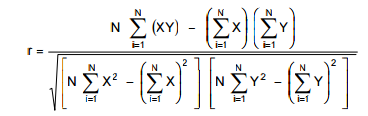
\includegraphics 
[scale=.7]{per.PNG}
\caption{COEFICIENTE DE CORRELACIÓN }
\end{figure}
donde N es el número de datos.
\begin{figure}[!htb]
La siguiente tabla muestra los datos registrados en una muestra  de
5 empresas para la recoleccion de datos sobre el proyecto. La razón empresa es (X) y las
preguntas hechas a cada uno de las empresas (Y)
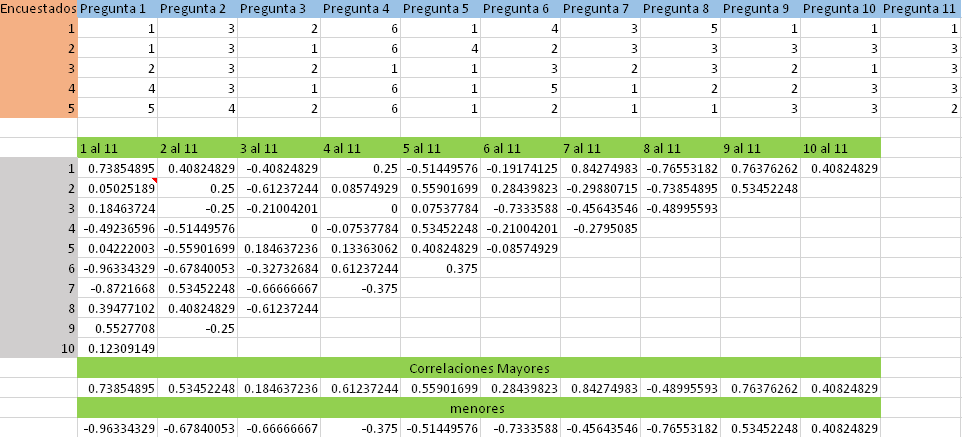
\includegraphics 
[scale=.3]{cor.PNG}
\end{figure}\\
Con anterior significa que, entre 0 y +1 cabe toda una gama de correlaciones positivas,
que serán tanto más directamente proporcionales, cuanto más se acerquen a +1.
Similarmente entre –1 y 0 cabe toda una gama de correlaciones negativas, que serán
tanto más inversamente proporcionales, cuanto más se acerquen a –1. Los
coeficientes de correlación, cuanto más cerca de cero, indican menor correlación. 
\\
Por lo tanto en las imagenes de abajo se podrán ver las correlaciones generadas con los resultados obtenidos en la tabla de arriba.
\begin{figure}[!htb]
En esta imagen se puede observar una gráfica correspondientes a las correlaciones mayores existes en todos los datos, existe una correlación entre ellas debido a que los datos estadísticos no varían en su escala de medición.
El coeficiente de correlación lineal es un número real comprendido entre menos −1 y 1.
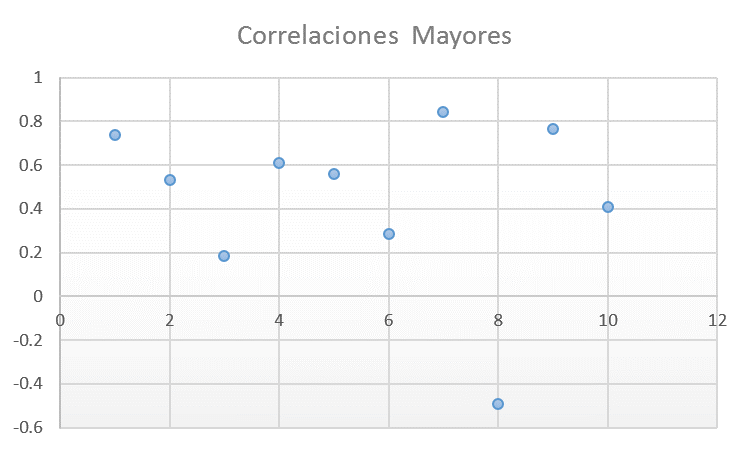
\includegraphics 
[scale=.6]{x1.png}
\end{figure}\\

\begin{figure}[!htb]
En las imágenes que ahora veremos corrresponderan a las correlaciones de datos menores, esto debido a que  toma valores cercanos a 0 y la correlación es débil.
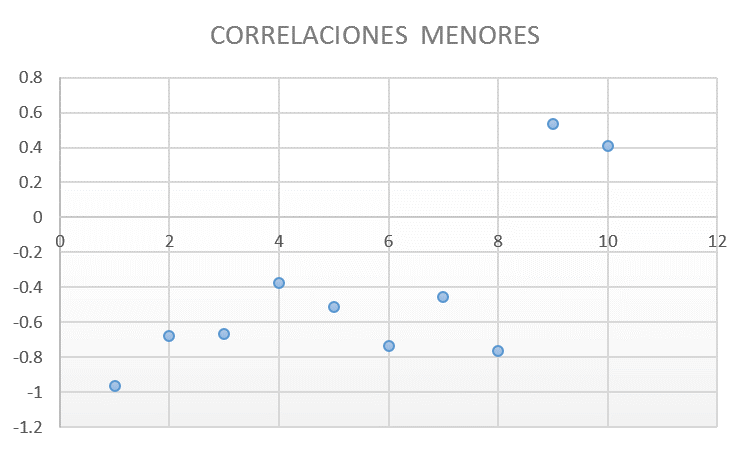
\includegraphics 
[scale=.6]{x2.png}
\end{figure}

\newpage
\section{Conclusión }
Para concluir con este informe de investigación, es importante mencionar y agradecer a las empresas que nos dieron la oportunidad de poder ver y realizar la entrevista de manera formal, esta investigación puede tener un gran impacto en la sociedad si se llegara a aplicar o darle seguimiento como debe de ser, hoy en día las calles no cuentan con ningún tipo de seguridad ni vigilancia, es por ello que la realización de este proyecto implementado a hacia esa área puede funcionar, llevando un control sobre ellas, y de igual forma poder localizar y ubicar a las personas que cometen algún délito, y de esa manera también se puede buscar a personas desaparecidas o personas que están siendo buscadas por la ley, como se mencionó al principio, se pretende crear u obtener una base de daos en la cual estén almacenados las fotografías de cada una de las personas desaparecidas o que están siendo buscadas por algún delito.
En este proyecto de investigación se obtuvieron resultados no muy favorables, ya que las empresas están acostumbrados al modelo tradicional en la que han venido trabajando, de igual forma les costaría tiempo en adaptarse a este nuevo modelo tecnológico, mas sin embargo comentaron que en un futuro se podría requerir de este tipo de tecnologías.
\section{Trabajos a futuros} \label{Trabajos a futuros}
Considerando que este proyecto es muy poco factible en las empresas, se puede orientar hacia otras áreas en donde podría haber financiamiento por parte de los interesados, como por ejemplo en el área de seguridad publica, esto beneficiara a toda la comunidad o a la población entrevistada, considero que el impacto sera muy grande y desde luego se adoptara hacia otras áreas, la seguridad ciudadana es un tema muy importante en estos días, ya que se viven robos, asaltos a mano armada, secuestros, peleas, et. Es por ello la importancia de este tipo de tecnologías en las calles.\\
Con respecto al trabajo realizado creo importante que se considere la forma de plantear las preguntas con especial cuidado, pues algunas pueden prestarse a confusión o los encuestados creen que hay más de un inciso que corresponde a su caso, por lo cual es bueno incluir una opción abierta,así como presento en el informe anterior, esto con la finalidad de que el entrevistado de un punto de vista mas especifico y de igual manera te enteras de cosas que ni tu mismo habías pensado.
\nocite{*}
\section{Referencias}
\bibliographystyle{compj}
\bibliography{ModellingBidders}
Balmelli Chuquisengo, L. E. (2006). Verificación de Identidad de Personas mediante. Sección de Electricidad y Electrónica, 62.\\
Cazorla Martínez, R. (2015). Software para la detección y el reconocimiento de rostros. TFG EN INGENIERÍA INFORMÁTICA, 10.\\
DE JESÚS RAMÍREZ, M., ALONSO, G., ÁVILA OROZCO, G., and MARTÍNEZ ÁVILA, L. (2010). Segmentación de imágenes a color para la IDENTIFICACIÓN AUTOMÁTICA ROSTROS utilizando FCM. Synthesis, 1-4.\\
GARCÍA GARCÍA, P. P. (2013). RECONOCIMIENTO DE IMÁGENES UTILIZANDO . 72.\\
Goit. (2014). Identificación AFIS y multibiométrica para proyectos de gran escala . VeriLook SDK, 3.\\
Gualdrón, O. E., Duque Suárez, O. M., and Chacón Rojas, M. A. (Noviembre 2013). DISEÑO DE UN SISTEMA DE RECONOCIMIENTO DE ROSTROS MEDIANTE LA HIBRIDACIÓN DE TÉCNICAS DE RECONOCIMIENTO DE PATRONES, VISIÓN ARTIFICIAL E IA, ENFOCADO A LA SEGURIDAD E INTERACCIÓN ROBÓTICA SOCIAL. 16 -28.\\
Llorente, A. (22 de Enero, de 2014). AirLive. Cámaras con reconocimiento facial , pág. 1.\\
López Sandoval, A. E., Mendoza Martínez, C., Reyes Cruz, L. Á., Rivas Araiza, E. A., Ramos Arreguín, J. M., and Pedraza Ortega, J. C. (Mayo 2015). Sistema de Autenticación Facial mediante la. mecamex, 53 – 64.
Ruiz Marín, M., Rodriguez Uribe, J. C., andand Olivares Morales, J. C.\\ (2009). Revista Avances en Sistemas e Informática . Una mirada a la biometria , 29-38.


\end{document}